% This is a sample document using the University of Minnesota, Morris, Computer Science
% Senior Seminar modification of the ACM sig-alternate style to generate a simple annotated
% bibliography. The idea is that this document is fairly short, consisting of a brief description
% of your sources and how you intend to use them (or not). Most of the ``content'' of the
% generated document comes from the bibliography file, including the notes field which will
% provide the annotations.

% See https://github.com/UMM-CSci/Senior_seminar_templates for more info and to make
% suggestions and corrections.

\documentclass{sig-alternate}
\usepackage{amsmath}
\usepackage{verbatim}

\begin{document}

% --- Author Metadata here ---
%%% REMEMBER TO CHANGE THE SEMESTER AND YEAR
\conferenceinfo{UMM CSci Senior Seminar Conference, December 2013}{Morris, MN}

\title{Zero Knowledge Compilers}

\numberofauthors{1}

\author{
% The command \alignauthor (no curly braces needed) should
% precede each author name, affiliation/snail-mail address and
% e-mail address. Additionally, tag each line of
% affiliation/address with \affaddr, and tag the
% e-mail address with \email.
\alignauthor
John T. McCall\\
	\affaddr{Division of Science and Mathematics}\\
	\affaddr{University of Minnesota, Morris}\\
	\affaddr{Morris, Minnesota, USA 56267}\\
	\email{mcca0798@morris.umn.edu}
}

\maketitle

\begin{abstract}
Zero knowledge protocols have useful applications in cryptography,
however they are usually designed by hand. They can be difficult to
design correctly, and it can be easy to make mistakes, as zero knowledge 
protocols are complex structures. Even if they are designed perfectly,
a programmer tasked with implementing it could find themselves in over
their head, especially if they lack a deep cryptographic background.
The goal behind zero knowledge compilers is to help alleviate these
concerns. Using a zero knowledge compiler, one can simply input a proof
goal and the compiler will output an implementation of that goal in a
high level language, such as Java or C++. The compiler also guarantees
correctness of the protocol, which eliminates the risk of subtle mistakes
in either the design or the implementation of the protocol.

\end{abstract}

\keywords{Zero Knowledge Protocols, Compilers, Zero Knowledge Compilers, ZKPDL, ZKCrypt}

\section{Introduction}
	Zero knowledge protocols provide a way of proving that a statement is true
	without revealing anything other than the correctness of this claim. Zero
	knowledge protocols have practical applications in cryptography and
	are used in many applications. While some applications only exist
	on a specification level, a direction of research has produced real-world
	applications. One such example is Direct Anonymous Attestation (DAA),
	a privacy-enhancing mechanism for remote authentication of computing
	platforms, which has been adopted by the Trusted Computing Group (TCG).
	
	Traditionally, the design of practical zero knowledge protocols
	is done by hand. Designers use standard arguments and tricks which
	can be combined and repeated in various combinations to provide the 
	desired, secure, protocol. There are a few problems with this type
	of method however. The implementations tend to be time-consuming
	and error-prone. Minor changes in the protocol specification often
	lead to major changes in the implementation. The protocols are usually
	designed by cryptographers and implemented by software engineers. The
	cryptographers typically are not skilled in implementation matters and
	the software engineers typically have a hard time understanding the
	complexities of the zero knowledge protocols~\cite{Sigma:2009}. 

	Zero knowledge compilers help to alleviate these issues by providing
	a way to automatically generate zero knowledge protocols for a large
	class of proof goals. They allow developers to implement these protocols
	without having an in depth knowledge of cryptography and without having to
	worry about introducing security flaws in their implementations.

	In sections 2 and 3, I provide background on zero knowledge protocols and
	compilers respectively. In section 4, I talk about some concepts from
	cryptography that are needed in understanding the compilers.
	In section 5, I talk about three different implementations of a zero knowledge 
	compiler. Finally, in section 6, I talk about electronic cash, an application 
	of zero knowledge protocols.

\section{Zero Knowledge Protocols}
	Zero knowledge protocols, also referred to as zero knowledge proofs, are a type
	of protocol in which one party, called the \textit{prover}, tries to convince the 
	other party, called the \textit{verifier}, that a given statement is true. Sometimes
	the statement is that the prover possesses a particular piece of information. This
	is a special case of zero knowledge protocol called a \textit{zero knowledge proof
	of knowledge}~\cite{Wiki}. Formally, a zero knowledge proof is a type of interactive
	proof.
	
	An interactive proof system is an interaction between a
	\textit{verifier} executing a probabilistic polynomial-time strategy and
	a \textit{prover} which executes a computationally unbound strategy.
	satisfying the following properties:
			
	\begin{itemize}
		\item \textit{Completeness}: If the statement being proved is true, an
		honest verifier (a verifier correctly following the protocol) will be
		convinced after interacting with an honest prover.
			
		\item \textit{Soundness}: If the statement is false, no prover, either
		honest or dishonest, will be able to convince an honest verifier, except
		with a small probability.
	\end{itemize}
	
	For an interactive proof to be a zero knowledge proof it must also
	satisfy the condition of \textit{zero knowledge}.	
	A proof is zero knowledge if any knowledge known by
	the prover or the verifier before performing the proof is the same
	as the knowledge known by either party after performing the proof.			
	In other words, no additional knowledge is gained by either party because
	of the proof. Another way of thinking about it is that the proof reveals 	
	zero knowledge~\cite{Survey}.

	\subsection{Examples}
	%Write an example using the Lyrics of Billie Jean
	
	Below are two examples of zero knowledge protocols. The
	first is a simple example which highlights how a zero knowledge
	protocol functions. The second is a more practical example,
	proving knowledge of a Hamiltonian cycle in a graph.
	
	\subsubsection{The Magic Cave}
	The classic example for zero knowledge protocols is the cave example.
	First presented in~\cite{Children:1987} and then restated
	in~\cite{Survey}, the cave example is the go-to example for learning
	zero knowledge protocols.

	Peggy has stumbled across a magical cave. Upon entering the cave
	there are two paths, one leading to the right and one leading to the
	left. Both paths eventually lead to a dead end, however Peggy has
	discovered a secret word that opens up a hidden door in the dead end,
	connecting both paths.

	Victor hears about this, and offers to buy the secret from Peggy.
	Before giving Peggy the money Victor
	wants to be certain that Peggy actually knows this secret word. How can
	Peggy (the prover) convince Victor (the verifier) that she knows the
	word, without revealing what it is?

	The two of them come up with the following plan. First, Victor will wait
	outside the cave while Peggy goes in. She will randomly pick either the
	right or the left path and go down it. Since Victor was outside he
	should have no knowledge of which path Peggy took. Then Victor will
	enter the cave. He will wait by the fork and shout to Peggy which
	path to return from. 
	
	Assuming that Peggy knows the word, she should be able to return down
	the correct path, regardless of which one she started on. If Victor 
	says to	return down the path she started on, she simply walks back. 
	If Victor says to return down the other path, she whispers the magic
	word, goes through the door, and returns down the other path.

	If Peggy doesn't know the word, there is a 50\% chance that Victor
	will choose the path she did not start down. If this happens there is
	no way that she can return down the correct path. The experiment should
	be repeated until Victor either discovers Peggy is a liar because she
	returned down the wrong path, or until he is sufficiently satisfied
	that she does indeed know the word.

	This is a zero knowledge protocol because it satisfies each of the three
	requirements. It satisfies completeness because	if Peggy knows the word
	she will be able to convince Victor. It is sound because if Peggy does not 
	know the word, she will not be able to convince Victor unless she was very
	lucky. Finally it is zero knowledge because if Victor follows the protocol
	he will not be able to learn anything besides whether or not Peggy knows 
	the word.
	
	\subsubsection{Hamiltonian Cycles}
	A more practical example is proving that one knows a Hamiltonian
	cycle for a graph, without revealing what the cycle is. Before
	going into the example we first need some graph theory background.
	A \textit{cycle} is a sequence of vertices, two consecutive vertices
	in the sequence are	adjacent (connected) to each other in the graph,
	which starts and ends at the same vertex. A \textit{Hamiltonian
	path}, is a sequence of vertices in which each vertex in the graph is
	listed exactly once. Finally, a \textit{Hamiltonian cycle}
	is a Hamiltonian path which is also a cycle. In other words it is a
	sequence of vertices which begins and ends with the same vertex, and
	each vertex in the graph is listed exactly once (aside from the first/last
	vertex)~\cite{Wiki:Hamiltonian}.
	
	\begin{figure}
	\centering
	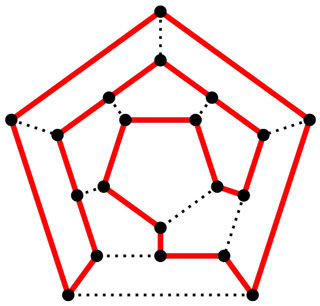
\psfig{file=HCycle.jpg, width=3.3in}
	\caption{An example of a Hamiltonian cycle. The solid line marks the path.
	Taken from~\cite{Wiki:Hamiltonian}.}
	\label{fig:HCycle}
	\end{figure}
	
	For a large enough
	graph, finding a Hamiltonian cycle is infeasible. In fact this problem, 
	is \textit{NP-complete}. NP-complete problems have the property that
	any known solution can be efficiently verified, however there is no known
	efficient way to find said solution. The time required to solve an 
	NP-complete problem increases rapidly as the size of the problem grows.
	Using current computing power, even moderately sized problems can take 
	billions of years to solve.
	
	Another important definition is that of graph isomorphism. An
	isomorphism, $f:V(G) \rightarrow V(H)$, of graphs $G$ and $H$ is a 
	bijection between the vertex
	sets of $G$ and $H$ such that any two vertices $u$ and $v$ of $G$ are
	adjacent in $G$ if and only if $f(u)$ and $f(v)$ are adjacent in $H$.
		
	Now that we have defined a Hamiltonian cycle, we can set up the example.
	Here the prover, $P$, knows a Hamiltonian Cycle for a graph, $G$. The
	verifier, $V$, has knowledge of $G$ but not the cycle. For $P$ to show
	$V$ that they know the cycle, they must perform several rounds of the 
	following protocol.
	
	\begin{itemize}
		\item At the beginning of each round, $P$ constructs $H$, graph which
		is isomorphic to $G$. It is simple to translate a Hamiltonian cycle
		between two isomorphic graphs, so since $P$ knows a Hamiltonian cycle
		for $G$ they must know one for $H$ as well.
		
		\item $P$ commits to $H$, either using a cryptographic commitment
		scheme or some other method. Doing this means that $P$ cannot change
		$H$, and at the same time $V$ has no knowledge of $H$.
		
		\item $V$ then randomly asks $P$ to do one of two things. Either show
		the isomorphism between $H$ and $G$, or show a Hamiltonian cycle in $H$.
		
		\item If $P$ was asked to show that the two graphs are isomorphic, they
		start by revealing $H$ to $V$. They also provide the vertex translations
		which map $G$ to $H$. $V$ can then verify that the two graphs are isomorphic.
		
		\item If $P$ was asked to show a Hamiltonian cycle in $H$, they first 
		translate the cycle from $G$ onto $H$. They then reveal to $V$ the 
		edges of $H$ which are a part of the Hamiltonian cycle. This is
		enough for $V$ to verify that $H$ contains a Hamiltonian cycle.
	\end{itemize}
	
	This protocol is complete because if $P$ is an honest prover, they can easily
	answer either question asked by $V$ by either providing the isomorphism which
	they have, or by applying the isomorphism to the cycle in $G$ to demonstrate
	a Hamiltonian cycle. This protocol is sound because if $P$ doesn't know the
	cycle, they can either generate a graph isomorphic to $G$ or a Hamiltonian
	cycle for another graph, but they cannot do both since they doesn't know a
	Hamiltonian cycle for $G$. With a reasonable number of rounds it is
	unrealistic for $P$ to fool $V$ in this manner.	This protocol is zero knowledge 
	because in each round $V$ will only learn either the isomorphism of $H$ to $G$
	or a Hamiltonian cycle in $H$. $V$ would need both pieces of information in
	order to reconstruct the Hamiltonian cycle in $G$. Therefore, as long as $P$
	can generate a distinct $H$ each round, $V$ will never discover the cycle in $G$.
	

\section{Compilers}
	Fundamentally, what a compiler does is translate one language into
	another. For example, a C++ compiler will take a C++ program as input and
	will output machine code. There are many different types of
	compilers, single-pass compilers, multi-pass, load-and-go, debugging compilers,
	optimizing compilers, and many combinations of these~\cite{Compiler:1986}.
	
	The first compilers started to appear in the 1950s. Much of the early work
	dealt with translating arithmetic formulas into machine code. At the time
	compilers were notoriously difficult to implement, for instance it took
	18 staff-years to implement the first Fortran compiler. Various languages,
	programming	environments, and tools have been developed since then which
	make implementing a compiler considerably easier.
	
	There are two parts to compilation, analysis and synthesis. Analysis breaks
	up the source into pieces and creates an intermediate representation, usually
	a syntax tree, of the program. Synthesis constructs the target program from
    the representation.
    
    It is difficult to implement a zero knowledge protocol due to their
	subtleties. For this reason work has gone into
	developing zero knowledge compilers. A zero knowledge compiler is a
	compiler which takes a proof goal as its input language
	and outputs an implementation of a zero knowledge proof.
    
    The compilers discussed in this paper take, as input, an abstract proof 
    specification or proof-goal, written in languages designed specifically 
    for this problem, and output an implementation of the given specification in
    a high-level language, usually C++ or Java.
    
    %% Add a picture of a Syntax Tree Here?
    
\section{Zero Knowledge Compilers}
	Before discussing the three different zero knowledge compilers we
	require the necessary background. First, I will go over some
	mathematical concepts used in the proofs and compilers.
	After that, I will talk about the common notation used to describe
	zero knowledge proofs. Once familiar with that we can then begin
	discussing the three compilers.
	
	\subsection{Background and Notation}
	A \textit{group}, in a mathematical sense, is a set, $G$ paired with an 
	operation, $\odot$, which combines any two elements (of the set) to form 
	another element. A group is denoted by: $(G, \odot)$. In order for a set
	and operation to be a group it must meet four requirements. The set must
	be closed under that operation, in other words for all $a, b$ in $G, a
	\odot b$ must also be in $G$. The operation must be associative, so for
	all $a, b$ in $G, (a \odot b) \odot c = a \odot (b \odot c)$. There must
	be an identity element, $e$ in $G$, such that for every element $a$ in $G$
	the equation $e \odot a = a \odot e = a$ is true. Finally, there must be
	an inverse element, so for each $a$ in $G$, there exists an element $b$ in
	$G$ such that $a \odot b = b \odot a = e$. An example of a group is the
	integers with addition, denoted $(\mathbb{Z}, +)$. This is a group because
	addition is closed and associative in the integers, it has an identity
	element (0), and each element of the integers has an inverse (negative 
	that element).
	
	A \textit{preimage}, or \textit{inverse image} of a function, $f:A \rightarrow B$, 
	is the set of all elements $a$ in $A$ such that $f(a)$ is in $B$. For example,
	if $f(x) = x^{2}$ then the preimage of $\{4\}$ would be $\{-2, 2\}$ because those
	are all the elements which equal 4 after the function is applied to them.
	
	A mapping $\phi : G \rightarrow H$ from an additive group $(G, +)$ into a
	multiplicative group $(H, \cdot)$ is called a \textit{homomorphism} if and
	only if for all $a, b$ in $G$ the following equation holds: $\phi(a + b) =
	\phi(a) \cdot \phi(b)$~\cite{Sigma:2009}.
	
	We will use notation described in~\cite{Sigma:2009} to denote zero knowledge
	proofs. An example of this notation is as follows:
	
	\begin{center}
		$\text{ZKP}[(\omega_{1},\omega_{2}):x_{1} = \phi_{1}(\omega_{1}) \land  x_{2} = \phi_{2}(\omega_{2}) \land \omega_{1} = a\omega_{2}]$ 
	\end{center}
	
	What this means is \textit{"proof of knowledge of $w_{1}, w_{2}$ such that 
	$x_{1} = \phi_{1}(\omega_{1}), x_{2} = \phi_{2}(\omega_{2})$ and $\omega_{1} = a\omega_{2}$}.
	The convention is that knowledge of variables listed before the colon
	must be proven, whereas knowledge of all other variables is
	assumed to be known by both the prover and the verifier. Another thing
	to note is that this is the notation for a \textit{proof-goal}, not
	a protocol. A proof-goal describes what has to be proven, and there may
	be several different protocols for the same proof-goal.

	\subsection{Sigma-Protocols}
	% I want to touch this area up and make it more clear just what Sigma
	% Protocols are. I also want to talk about the compiler that the authors made
		Bangerter et al. present in~\cite{Sigma:2009} a language and compiler
		which generates sound and efficient zero knowledge proofs of knowledge
		based on $\Sigma$-Protocols.	
	
		$\Sigma$-Protocols are the basis of essentially all efficient zero knowledge
		proofs of knowledge used in practice today. $\Sigma$-Protocols are a class of
		three-move protocols, meaning three messages are exchanged between the prover
		and the verifier. First the prover, $P$, sends a \textit{commitment} $t$ to the
		verifier, $V$. $V$ then responds with a random \textit{challenge} $c$ from a 
		predefined set of challenges $C$. $P$ computes a \textit{response} $s$ and sends
		it to $V$ who then decides whether to accept or reject the proof.
		
		Bangerter et al's compiler is used to generate implementations of proofs
		of knowledge of preimages under homomorphisms. An arbitrary number of these
		proofs can be combined by using the boolean ``AND" and ``OR" operators.
		The compiler can handle the class of proof goals consisting of
		all expressions of the forms:
		
		\begin{equation*}
		\text{ZKP}[(\omega_{1},...,\omega_{m}):\bigvee\bigwedge y_{i} = \phi_{i}(\omega_{i})]
		\end{equation*}
		or
		\begin{equation*}
		\text{ZKP}[(\omega_{1},...,\omega_{m}):\bigwedge y_{i} = \phi_{i}(\omega_{1},...,\omega_{m})\land HLR(\omega_{1},...,\omega_{m})]
		\end{equation*}
		
		The first equation can be expressed
		as an arbitrary monotone boolean formula, in other words a boolean formula
		with an arbitrarily number of $\land$ and $\lor$ symbols and has predicates of
		the form $y_{j} = \phi_{j}(\omega_{j}).$ Also, in both of the above equations
		linear relations can be proven \textit{implicitly}: as an example, we can
		see that $\text{ZKP}[(\omega_{1},\omega_{2}):y = \phi(\omega_{1},\omega_{2}) \land \omega_{1} = 2\omega_{2}]$
		is equivalent to $\text{ZKP}[(\omega):y = \phi(2\omega,\omega)]$ by setting $\omega:=\omega_{2}$.
		
		The input language of this compiler requires Declarations of any
		algebraic objects involved (such as: groups, elements, homomorphims, and
		constants), Assignments from group elements to the group
		they live in, and Definitions of homomorphims. Once all of these
		have been set up, the protocol to be generated is specified in the
		SpecifiyProtocol [...] block.
		
		The compiler outputs Java code for the $\Sigma$-Protocol, which
		can then be used in other applications. Alternatively the compiler
		can output \LaTeX~documentation of the protocol if told to do so.
		
	\subsection{ZKCrypt}
		Almeida et al. present, in~\cite{ZKCrypt:2012}, ZKCrypt, an optimizing cryptographic
		compiler. Similar to the above language, ZKCrypt is also based on $\Sigma$-Protocols.
		Using recent developments, ZKCrypt can achieve ``an unprecedented level of confidence
		among cryptographic compilers"~\cite{ZKCrypt:2012}. Specifically these developments are:
		\textit{verified compilation}, where the correctness of a compiler is proved once-and-for-all,
		and \textit{verifying compilation}, where the correctness of a compiler is checked on
		each run. ZKCrypt uses these techniques by implementing two compilers, one of which
		is a verified compiler and the other a verifying compiler, both of which are used when
		implementing a zero knowledge protocol. The verified compiler generates
		a reference implementation. The verifying compiler outputs an optimized implementation
		which is provably equivalent to the reference implementation. 
		
		ZKCrypt has four main parts to its compilation process. They are: resolution, verified
		compilation, implementation, and generation. The first phase, resolution, takes a
		description of a proof goal, G, as input. This description is written in the the standard
		notation for zero knowledge proofs. G is converted into a resolved goal
		G$_{\textrm{res}}$, in which
		high-level range restrictions are converted into proofs of knowledge of preimages under
		homomorphisms. The next phase, verified compilation, takes G$_{\textrm{res}}$ and 
		outputs I$_{\textrm{ref}}$,
		a reference implementation in the language of CertiCrypt, which is a toolset used in
		the construction and verification of cryptographic proofs. At this point a 
		once-and-for-all proof of correctness is done to guarantee that I$_{\textrm{ref}}$
		satisfies the desired security properties. The implementation phase
		also takes G$_{\textrm{res}}$ as input however it outputs I$_{\textrm{opt}}$, an
		optimized implementation. An equivalence checker is used to prove that I$_{\textrm{ref}}$
		and I$_{\textrm{opt}}$ are semantically equivalent. In the final phase, generation,
		the optimized implementation is converted into C and Java implementations of the
		protocol.
				
	\subsection{ZKPDL}
		Meiklejohn et al. provide a language called the Zero-Knowledge Proof Description
		Language (ZKPDL)~\cite{ZKPDL:2010}. This language makes it much easier for both
		programmers and 	cryptographers to implement protocols. The authors aim to enable
		secure, anonymous electronic cash (e-cash) in network applications.
		
		This language provides two main benefits. Firstly, the programmer no longer 
		has to worry about implementing cryptographic primitives, efficient mathematical
		operations, or generating and processing messages. ZKPDL allows the user to
		specify the protocol similarly to how it would be specified in a theoretical
		description. Secondly, the library makes performance optimizations based on an
		analysis of the protocol description. 
		
		Similarly to the language above, ZKPDL makes use of $\Sigma$-Protocols.
		However, ZKPDL doesn't implement them directly. Instead, they use the 
		Fiat-Shamir heuristic, which transforms $\Sigma$-protocols into non-interactive
		zero-knowledge proofs.
		
		The authors also provide an interpreter for ZKPDL, implemented in C++, which
		preforms one of two actions depending on the role of the user. On the prover
		side it outputs a zero knowledge proof. On the verifier side it takes a proof
		and verifies its correctness. Regardless of the role of the user, the program
		given to the interpreter is the same. The interpreter also performs a number of
		optimizations including precomputations, caching, and translations to prevent
		redundant proofs. 

		Two types of variables can be declared in this language: group objects
		and numerical objects. Group generators can also be declared but this 
		is optional. Numerical objects can either be declared in a list of variables
		or by having their type specified by the user. Valid types are: \texttt{element},
		\texttt{exponent}, and \texttt{integer}. 		
		
		A program written in this language is split into two blocks: a computation block,
		and a proof block. Both blocks are optional, if the user is only interested in the
		computation they can just write that. Alternatively, if the user has all the computations
		done they can just write the proof block. 
		
		The computation block can be further split into two blocks: the \texttt{given} block
		and the \texttt{compute} block. In the \texttt{given} block the parameters are specified
		as well as any values which are necessary for the computation that the user has already
		computed. The \texttt{compute} block carries out the given computations. There are two
		types of computations: picking a random value, and defining a value by setting it
		equal to the right-hand side of an equation.
		
		The proof block is made up of three blocks: the \texttt{given} block, the 
		\texttt{prove knowledge of} block, and the \texttt{such that} block. In the
		\texttt{given} block the proof parameters are specified as well as any inputs
		known publicly to both the prover and the verifier. The inputs known privately to
		the prover are specified in the \texttt{prove knowledge of block}. In the 
		\texttt{such that} block the relations between all the values are specified.
		The zero-knowledge proof will be a proof that all these relations are satisfied.
		
	    
	    \begin{comment}
		\begin{verbatim}
		computation: // compute values required for proof
		  given: // declarations
		    group: G = <g. h>
		    exponents in G: x[2:3]
		  compute: // declarations and assignments
		    random exponents in G: r[1:3]
		    x_1 := x_2 * x_3
		    for(i, 1:3, c_i := g^x_i * h^r_i)
		    
		proof:
		  given: // declarations of public values
		    group: G = <g, h>
		    elements in G: c[1:3]
		    for(i, 1:3, commitment to x_i: c_i = g^x_i * h^r_i)
		  prove knowledge of: // declarations of private values
		    exponents in G: x[1:3], r[1:3]
		  such that: // protocol specification; i.e. relations
		    x_1 = x_2 * x_3
		\end{verbatim}
		
		In this example, the authors are proving that the value $x_{1}$ contained within
		the commitment $c_{1}$ is the product of $x_{2}$ and $x_{3}$ which are contained
		in $c_{2}$ and $c_{3}$ respectively. Because both blocks are optional, they are
		considered independent from each other, so a lines are repeated between the two.
		\end{comment}

\begin{comment}
\section{Applications}
	In general, zero knowledge protocols have many applications. Authentication systems,
	electronic voting, electronic ticketing, Direct Anonymous Attestation (DAA), and
	Off-the-Record messaging~\cite{ZKCrypt:2012, ZKPDL:2010} are just a few examples.
	The applications that will be focused on in this paper are electronic cash, and
	deniable authentication.
	
	\subsection{Electronic Cash}
	Electronic Cash, or e-cash, is an electronic currency. E-cash maintains the buyer's
	anonymity, unlike a debit or credit card that is used to purchase something 
	electronically. Bitcoins are a recent example of an e-cash system.
	
	Okamoto and Ohta describe the ideal electronic cash system in~\cite{Ecash:1991}.
	The ideals are as follows:
	
	\begin{enumerate}
		\item \textit{Independence}: The security of electronic cash cannot depend on any
		physical condition. Then the cash can be transferred through networks.
		
		\item \textit{Security}: The ability to copy (reuse) and forge the cash must be
		prevented.
		
		\item \textit{Privacy (Untraceability)}: The privacy of the user should be
		protected. That is, the relationship between the user and their purchases must
		be untraceable by anyone.
		
		\item \textit{Off-line payment}: When a user pays the electronic cash to a shop, 
		the procedure between the user and the shop should be executed in an off-line
		manner. That is, the shop does not need to be linked to the host in user's
		payment procedure.
		
		\item \textit{Transferability}: The cash can be transferred to other users.
		
		\item \textit{Dividability}: One issued piece of cash worth value $C$ (dollars)
		can be subdivided into many pieces such that each subdivided piece is worth any
		desired value less than $C$ and the total value of all the pieces is equivalent
		to $C$.
	\end{enumerate}
	
	Almeida et al. describe briefly in~\cite{ZKCrypt:2012} how ZKCrypt can be used to
	generate a proof for proving the identity of the user when withdrawing money from
	a bank account. The user has to prove they have a secret key in order to successfully
	withdraw money. 
	
	The authors state the proof goal as:
	\begin{align*}
	ZPK\left[(u_{1}, u_{2}): I = g^{u_{1}}_{1}g^{u_{2}}_{2}\right].
	\end{align*}
	In this goal, $I, g_{1}, g_{2} \in \mathbb{Z}^{*}_{p}$ such that ord $g_{1}$ = ord
	$g_{2}$ = $q$, where $q|(p - 1)$ and $p, q \in \mathbb{P}$. The secrets $u_{1}, u_{2}$
	are elements of $\mathbb{Z}_{q}$. A single instance of the $\Sigma^{\Phi}$-protocol
	is enough to realize this goal.
	
	Meiklejohn et al. also give this example, a user proving their identity to the bank,
	implemented in ZKDPL. The program for this looks like: 
	\begin{verbatim}
	proof:
	  given:
	  	group: cashGroup = <f, g, h, h1, h2>
	  	elements in cashGroup: A, pk_u
	  	  commitment to sk_u: A = g^sk_u * h^r_u
	  prove knowledge of:
	  	exponents in cashGroup: sk_u, r_u
	  such that:
	  	pk_u = g^sk_u
	  	A = g^sk_u * h^r_u
	\end{verbatim}
	
	When the bank has verified this proof, the bank and the user will run a protocol
	which defines a wallet which contains $W$ coins, where $W$ is a system-wide
	public parameter. When a user spends a coin, it is split up into two parts: an
	endorsed part and an unendorsed part. Separately the two parts are worthless, but
	together the coin becomes valid. First the unendorsed part is sent to the vendor
	who proves its validity. The vendor then sends what the buyer has purchased. The
	buyer sends the endorsed portion of the coin to the vendor upon receiving their
	product.
	
	\end{comment}

\section{Conclusion}
	Zero knowledge protocols are becoming more and more important in today's society. 
	Because they can be incredibly complex and take a while to implement, it is important 
	that there are efficient and secure ways of implementing them. In this paper we discussed
	three zero knowledge compilers and thier associated input languages. Each of these compilers
	hopes to aid in the implementation of zero knowledge protocols by offering a way for
	developers to easily generate an implementation of a given proof goal.
	
	\subsection{Current State and Future Work}
	Currently, all three of the compilers presented in this paper have
	been implemented in some form. The compiler outlined in~\cite{Sigma:2009}
	has native support for two groups and allows users to define their own
	groups. Future features of the compiler includes supporting efficient
	proofs in hidden-order groups, as well as the automatic transformation
	of the generated $\Sigma$-protocols into non-interactive zero knowledge
	proofs.
	
	ZKCrypt has been implemented and applied to several cryptographic
	problems, including electronic cash and deniable authentication.
	Future work for the ZKCrypt compiler includes verifying the last
	stage of the compiler chain, code generation. With this verified,
	the whole compilation process will be verified correct.
	
	ZKPDL has also been implemented and has been applied to problems
	such as electronic cash and verifiable encryption. Future work being
	considered for ZKPDL includes adding more cryptographic primitives,
	such as: encryption, signatures, and hash functions. Another interesting
	possibility would be the analysis of ZKDPL programs by providing automatic
	verification of protocols and the ability to identify security errors.
	Work is also being done to increase performance on multicore architectures
	by analyzing dependencies among expressions evaluated by the interpreter.	
	
	\subsection{Acknowledgments}
	// TODO

% The following two commands are all you need to
% produce the bibliography for the citations in your paper.
\bibliographystyle{abbrv}
% annotated_bibliography.bib is the name of the BibTex file containing 
% all the bibliography entries for this example. Note that you *don't* include the 
% .bib ending
% in the \bibliography command.
\bibliography{annotated_bibliography}

% You must have a ".bib" file and remember to run:
%     pdflatex bibtex pdflatex pdflatex
% in order to see all the citation references correctly.

\end{document}
